\subsection{Βήμα 1 - Κατηγοριοποίηση δεδομένων}
\begin{figure}[H]
    \begin{javacode}
    categories = new HashMap<>();
    getMovieInsights(long id, BaseWrapper<?> o) {
        if (categories.containsKey(id)) {
            return categoriess.get(id);
        }
        IMovieInsightsWrapper wrapper = createMovieInsightsWrapper(o);
        categories.put(id,wrapper);
        return wrapper;
    }
    getMovieInsightObjectsOptimized(Movie movie) {
     // return set of getMovieInsights(...)
    }
    categorizeData(Movie movie) {
        Set<IMovieInsightsWrapper> miSet = getMovieInsightObjectsOptimized(movie);
        miSet.forEach(wrapper -> {
            wrapper.submitMovie(movie);
        });
    }
    Lists
      .partition(dto.movies, 1000)
      .forEach(chunk -> {
         chunk.forEach(this::categorizeData);
      });
    \end{javacode}
    \caption{Σειριακή κατηγοριοποίηση με HashMap}
   \label{code:categorieSerialWithHM}
\end{figure}
Ο Αλγόριθμός κατηγοριοποίησης συλλέγει τα δεδομένα, τα προσθέτει στις ανάλογες κατηγορίες, δημιουργεί τις κατηγορίες αν δεν υπάρχουν, και ετοιμάζει τα δεδομένα για τον τελικό υπολογισμό.

Υπήρξαν πολλές αναθεωρήσεις του αλγορίθμου μέχρι την τελική του έκδοση. Οι περισσότερες αφορούσαν βελτιστοποιήσεις απόδοσης. 

Ο Αρχικός κώδικας (βλ σχήμα: \ref{code:categorieSerialWithHM}) ήταν αρκετά απλός. Είχε HashMaps για την αποθήκευση των δεδομένων ανά κατηγορία, και γινόταν συνεχώς έλεγχοι για το αν υπήρχαν  τα δεδομένα. Αν όχι τα δημιουργούσε αλλιώς τα μορφοποιούσε.
Αρχικά ο κώδικας έτρεχε σειριακά, καθώς όμως αυξανόταν τα δεδομένα ανέβαινε εκθετικά και ο χρόνος κατηγοριοποίησης τους. Για παράδειγμα για 1000 ταινίες μαζί με τους ηθοποιούς , εταιρίες και χώρες παραγωγής και είδη ταινιών τους, έκανε 25 λεπτά για την ολοκλήρωση της κατηγοριοποίησης. Για 5000 ταινίες έκανε πάνω από 8 ώρες. 
Ο κώδικας ξαναγράφτηκε (βλ σχήμα: \ref{code:categorieParallelWithCHM}) για να τρέχει με παραλληλισμό. Έτσι κάποια βασικά στοιχεία άλλαξαν, όπως τα HashMaps έγιναν ConcurrentHashMaps και κάποια άλλα κομμάτια έγιναν Synchronize για να υπάρχει Thread Safety. Το αποτέλεσμα αυτών των αλλαγών ήταν η κατηγοριοποίηση 8000 ταινιών, συνυπολογίζοντας και τα λοιπά σχετικά στοιχεία, να ολοκληρώνεται εντός 25 λεπτών.

\begin{figure}[h]
    \begin{javacode}
    categories = new ConcurrentHashMap<>();
    categorizeData(Movie movie) { // ...
        miSet.parallelStream().forEach // ...
    }
    Lists
      // ...
         chunk
            .parallelStream().forEach // ...
      
    \end{javacode}
    \caption{Παράλληλης κατηγοριοποίηση με ConcurrentHashMap}
   \label{code:categorieParallelWithCHM}
\end{figure}

Αλλά ακόμα πιο γρήγορα φάνηκε ενα πρόβλημα απόδοσης που κρυβόταν απο την 
πρώτη υλοποίηση. Τα HashMaps. 
%Στην πορεία εμφανίστηκε ένα πρόβλημα απόδοσης, το οποίο δεν ήταν ορατό κατά την πρώτη υλοποίηση, και το οποίο αφορούσε τα HashMaps.
Ενω δίνουν με μεγάλη ευκολία, ένα Indexer για την αποθήκευση key-value pairs, έχουν μεγάλο performance-pentalty όταν αρχίζει και μεγαλώνει ο όγκος των ανατεθειμένων δεδομένων και το πρόβλημα μεγεθύνεται ακόμα πιο πολύ όταν είναι και ConcurrentHashMaps λόγω των ελέγχων που γίνονται. Ένα δείγμα 30000 ταινιών έκανε πάνω από 4.5 ώρες για να κατηγοριοποιήσει.

Κάτι έπρεπε να αντικαταστήσει τα HashMaps. Στην τελική έκδοση του αλγόριθμου (βλ σχήμα: \ref{code:categorieParallelWithArr}) τα HashMaps αντικαταστάθηκαν με τα Native Arrays. Η επιλογή αυτή είχε ιδιαιτέρως θετικό αντίκτυπο στην ταχύτητα της κατηγοριοποίησης.
Συγκριτικά με τη χρήση ConcurrentHashMaps, όπου η κατηγοριοποίηση 30.000 ταινιών εκτελούνταν σε 4,5 ώρες, ο ανανεωμένος αλγόριθμος κατηγοριοποίησε 30000 ταινίες σε μόλις 8 λεπτά. 

\begin{figure}[h]
    \begin{javacode}
    creditsArray = new MovieInsightsPersonWrapper[dto.maxPersonId][CreditRole.getSize()];
    companiesArray = new MovieInsightsCompanyWrapper[dto.maxCompanyId];
    countriesArray = new MovieInsightsCountryWrapper[dto.maxCountryId];
    genresArray = new MovieInsightsGenreWrapper[dto.maxGenreId];
    
    getMovieInsights(long id, BaseWrapper<?> o, IMovieInsightsWrapper[] array) {
        synchronized (array) {
            IMovieInsightsWrapper wrapper;
            if ((wrapper = array[(int) id]) == null) {
                array[(int) id] = wrapper = createMovieInsightsWrapper(o);
            }
            return wrapper;
        }
    }
    \end{javacode}
    \caption{Παράλληλη κατηγοριοποίηση με Arrays}
   \label{code:categorieParallelWithArr}
\end{figure}
Ο αλγόριθμος λοιπόν κατηγοριοποιεί τα δεδομένα όπως φαίνεται στο σχήμα \ref{flowchart:categorizeData} και αφού τελειώσει προχωράει στο βήμα 2 του υπολογισμού των δεδομένων.
\begin{figure}[H]
  \centering
  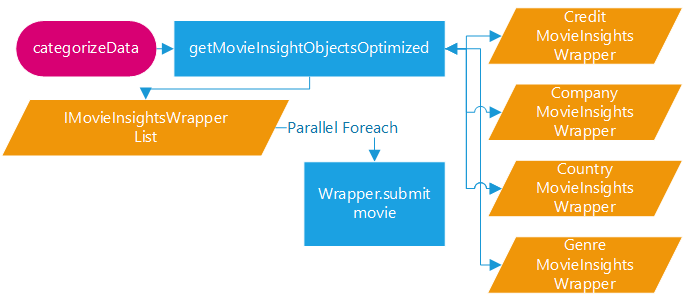
\includegraphics[width=150mm]{Chapters/5 - Architecture/MovieInsights/Images/categorizeData.png}
  \caption{Διάγραμμα ροής κατηγοριοποίησης δεδομένων}
  \label{flowchart:categorizeData}
\end{figure}